\documentclass[tcc2, pos-defesa, english, brazil]{packages/ufgrc}

\usepackage{rotating}
\usepackage[all,knot,arc,import,poly]{xy}

\usepackage{listings}
\usepackage{xcolor}
\usepackage[utf8]{inputenc}

\lstset{
    basicstyle=\ttfamily,
    keywordstyle=\color{blue},
    commentstyle=\color{green},
    stringstyle=\color{red},
    numbers=none,
    frame=single,
    tabsize=2,
    captionpos=b,
    language=C++
}

\titulo{Monitoramento das Emissões de CO2 na Agricultura: Desenvolvimento e Implementação de uma Rede de Nós Sensoriais Baseada em Redes Mesh}
\autor[JACINTO, W. B.]{Weleson Batista Jacinto}
\genero{M}
\orientador[Orientador]{Prof. Dr.}{Tércio Alberto Santos Filho}
\data{01}{01}{2026}

\membrobanca{Dr. Sergio Francisco da Silva}{Universidade Federal de Catalão}
\membrobanca{Dr. Ricardo Couto Antunes da Rocha}{Universidade Federal de Catalão}


% RESUMOS
% ---

% Resumo em PORTUGUÊS
% conter no máximo 500 palavras
% conter no mínimo 1 e no máximo 5 palavras-chave (obrigatoriamente separadas por vírgula)
\textoresumo[brazil]{O monitoramento das emissões de dióxido de carbono (CO2) é crucial para enfrentar as mudanças climáticas e promover a sustentabilidade na agricultura. O CO2, embora essencial para a fotossíntese, contribui para o aquecimento global quando suas concentrações aumentam devido a atividades humanas. Este estudo visa desenvolver e implementar um nó sensorial para monitoramento em tempo real das emissões de CO2 em áreas agrícolas, utilizando tecnologias de sensores e redes mesh com o protocolo ESP-MESH e microcontroladores ESP8266. O trabalho é dividido em várias seções: a introdução apresenta a importância do monitoramento de CO2 para mitigar as mudanças climáticas e destaca o papel do mercado de carbono. A fundamentação teórica aborda conceitos de monitoramento ambiental, tecnologias de sensores, emissões de CO2 na agricultura, mercado de carbono e redes mesh. A metodologia inclui a revisão bibliográfica, desenvolvimento do protótipo, configuração da rede de sensores, coleta e análise de dados, e proposição de medidas de mitigação. Os resultados esperados incluem a identificação de principais fontes de emissão e o desenvolvimento de modelos de estimativa de emissões. A pesquisa destaca a importância de tecnologias emergentes no monitoramento das emissões e sua contribuição para práticas agrícolas sustentáveis e políticas públicas eficazes.}{Emissões de CO2, Agricultura, Monitoramento, Mudanças climáticas, Nó sensorial}


% resumo em INGLÊS
% conter no máximo 500 palavras
% conter no mínimo 1 e no máximo 5 palavras-chave (obrigatoriamente separadas por vírgula)
\textoresumo[english]{Monitoring carbon dioxide (CO2) emissions is crucial for addressing climate change and promoting sustainability in agriculture. CO2, while essential for photosynthesis, contributes to global warming when its concentrations increase due to human activities. This study aims to develop and implement a sensor node for real-time CO2 emissions monitoring in agricultural areas, utilizing sensor technologies and mesh networks with the ESP-MESH protocol and ESP8266 microcontrollers. The work is structured into several sections: the introduction highlights the importance of CO2 monitoring for climate change mitigation and the role of the carbon market. The theoretical background covers environmental monitoring concepts, sensor technologies, CO2 emissions in agriculture, carbon market, and mesh networks. The methodology involves a literature review, prototype development, sensor network setup, data collection and analysis, and mitigation measures proposal. Expected results include identifying major emission sources and developing emission estimation models. The research emphasizes the importance of emerging technologies in emissions monitoring and their contribution to sustainable agricultural practices and effective public policies.}{CO2 emissions, Agriculture, Monitoring, Climate change, Sensory node}

\hypersetup{
    colorlinks=true
}

\begin{document}

\textual

\chapter{Introdução}
\label{chapter:introducao}
\section{Contextualização}

O dióxido de carbono (CO\textsubscript{2}) é um gás incolor e inodoro presente naturalmente na atmosfera e essencial para a vida na Terra. Na agricultura, o CO\textsubscript{2} é fundamental para o processo de fotossíntese, onde as plantas o utilizam para produzir açúcares e oxigênio \cite{ipcc2019land}.

Contudo, o aumento das concentrações de CO\textsubscript{2} causado pelas atividades humanas contribui significativamente para o aquecimento global, intensificando as mudanças climáticas, a alteração nos eventos climáticos e os padrões de precipitação. Esse aumento da temperatura no planeta resulta na acidificação dos oceanos, na perda de biodiversidade e na desertificação, além de impactar negativamente a agricultura e a segurança alimentar \cite{ipcc2021ar6}. Outro ponto importante são as práticas agrícolas, como o desmatamento e o uso intensivo de fertilizantes, que intensificam as emissões de outros gases de efeito estufa, como o metano (CH\textsubscript{4}) e o óxido nitroso (N\textsubscript{2}O). Reduzir as emissões de CO\textsubscript{2} na agricultura é, portanto, essencial para garantir a sustentabilidade do planeta \cite{ipcc2014afolu}.

Nesse contexto, o mercado de carbono emerge como uma ferramenta para incentivar a redução das emissões de gases de efeito estufa. Ao atribuir um valor econômico ao CO\textsubscript{2} e outros gases, o mercado de carbono promove práticas agrícolas mais sustentáveis, permitindo que os produtores rurais participem ativamente na mitigação das mudanças climáticas \cite{worldbank2022carbon}. Esse mecanismo não só oferece incentivos financeiros para reduzir as emissões, mas também contribui para a conservação dos recursos naturais e a proteção dos ecossistemas. Integrar a agricultura a este mercado pode ser uma estratégia eficaz para alinhar a produção agrícola com as metas globais de redução de emissões, destacando a importância de práticas sustentáveis no setor \cite{unfccc2020markets}.

O monitoramento das emissões de dióxido de carbono é crucial para entender e mitigar os impactos das mudanças climáticas. A coleta contínua e a análise de dados permitem identificar as principais fontes de emissão e suas variações, facilitando o desenvolvimento de estratégias eficazes e a promoção de práticas agrícolas sustentáveis \cite{ipcc2014afolu}. Além disso, esses dados são fundamentais para a formulação de políticas públicas voltadas para a redução dos gases de efeito estufa.

Diversas tecnologias são empregadas no monitoramento ambiental, com potencial significativo de aplicação no contexto agrícola. Sensores projetados para medir a qualidade do ar detectam os gases de efeito estufa presentes no ambiente, fornecendo dados importantes para o monitoramento e análise das emissões. Redes mesh de sensores conectam múltiplos dispositivos de forma colaborativa, possibilitando a coleta e transmissão de dados de maneira eficiente e abrangente \cite{zhao2018wsn}. Tecnologias de comunicação sem fio, como o protocolo ESP-MESH utilizado com o módulo ESP8266, permitem a formação de redes mesh que facilitam a comunicação eficiente entre sensores e a transmissão de dados para análise e armazenamento \cite{espressif2024mesh}. Essa abordagem é especialmente útil em aplicações que exigem baixo consumo de energia e cobertura em áreas extensas, como no monitoramento ambiental de gases de efeito estufa. Além disso, essa tecnologia pode desempenhar um papel crucial na regulamentação do mercado de carbono no Brasil, que atualmente é realizada de forma voluntária.

Entretanto, a medição das emissões enfrenta desafios como a precisão dos sensores, que pode ser influenciada por condições ambientais variáveis, e a necessidade de cobertura e conectividade em áreas agrícolas extensas. Além disso, o armazenamento e a análise de grandes volumes de dados exigem sistemas robustos e técnicas avançadas para extrair informações úteis \cite{liu2018iot}.

Este estudo propõe desenvolver e implementar um nó sensorial para o monitoramento das emissões de CO\textsubscript{2} na agricultura. A proposta engloba a criação de um protótipo que integra sensores ambientais a uma rede de comunicação sem fio baseada no protocolo ESP-MESH do microcontrolador ESP8266, permitindo coleta e transmissão de dados. A rede será composta por nós distribuídos estrategicamente em áreas agrícolas, garantindo cobertura abrangente graças à possibilidade de comunicação sem fio e à capacidade do protocolo ESP-MESH de estabelecer conexão entre múltiplos dispositivos, sem depender de uma infraestrutura centralizada \cite{espressif2024mesh}. Essa característica é especialmente vantajosa em ambientes agrícolas, permitindo a instalação de nós sensoriais em lavouras, pastagens e florestas, mesmo em terrenos irregulares, formando uma malha auto-organizável adaptada à topografia local. A distribuição estratégica dos sensores possibilita o monitoramento de grandes extensões. Além disso, a solução apresenta potencial de escalabilidade para outros contextos, como áreas urbanas, priorizando baixo consumo de energia e robustez, alinhando-se às demandas por sustentabilidade e eficiência em diferentes setores.

\section{Objetivo principal}
O objetivo principal deste trabalho é desenvolver e implementar uma rede de nós sensoriais para monitoramento contínuo e autônomo das emissões de CO\textsubscript{2} em cultivos agrícolas.

\section{Objetivos específicos}
\begin{itemize}
    \item Projetar e construir unidades sensoriais autônomas para medição de CO\textsubscript{2}
    \item Implementar a rede de sensores em uma cultura agrícola específica
    \item Coletar e transmitir os dados ambientais para uma plataforma digital
    \item Desenvolver visualizações gráficas intuitivas dos dados coletados
\end{itemize}

\section{Justificativa}

Este estudo é justificado pela relevância do monitoramento das emissões de CO\textsubscript{2} na agricultura como instrumento para incentivar a mitigação das mudanças climáticas e para apoiar a criação de um mercado de carbono regulamentado no Brasil, uma vez que a medição fornecida pelos sensores trará maior transparência ao processo, permitindo a quantificação dessas emissões. A pesquisa concentra-se no desenvolvimento e implementação de tecnologias de sensores e comunicação para a obtenção de dados contínuos sobre as emissões de CO\textsubscript{2}.

O monitoramento das emissões é fundamental para compreender o impacto das práticas agrícolas no meio ambiente e para subsidiar o desenvolvimento de estratégias de mitigação adequadas. Este estudo busca oferecer uma solução prática e eficiente para a coleta e análise de dados de emissões, contribuindo para práticas agrícolas mais sustentáveis e para a formulação de políticas públicas voltadas ao controle de gases de efeito estufa.

\chapter{Fundamentação Teórica}
\label{chapter:fundamentacao}
\section{Contextualização}

O monitoramento das emissões de CO\textsubscript{2} é essencial para incentivar a sustentabilidade agrícola e mitigar os efeitos das mudanças climáticas. Além do CO\textsubscript{2}, outros gases de efeito estufa, como o metano (CH\textsubscript{4}) e o óxido nitroso (N\textsubscript{2}O), têm impacto significativo no meio ambiente. A ausência de métodos que garantam transparência aos produtores e órgãos reguladores para medir e controlar essas emissões compromete os esforços de promoção de práticas agrícolas sustentáveis e de redução da pegada de carbono, prejudicando a saúde do planeta.

A tecnologia desempenha um papel crucial nesse contexto. Sensores modernos permitem o monitoramento contínuo das emissões de CO\textsubscript{2} com custo relativamente baixo. Quando integrados a redes \emph{mesh} e microcontroladores, esses sensores viabilizam a coleta e a transmissão de dados, otimizando o controle das emissões. Essas ferramentas são fundamentais para que o setor agrícola atenda às regulamentações ambientais e aproveite oportunidades no mercado de carbono \cite{inpe23, mma21} 

Ao longo deste capítulo, discutiremos:

\begin{itemize}
    \item A importância do monitoramento das emissões de CO\textsubscript{2} na agricultura;
    \item As tecnologias de sensores disponíveis;
    \item Como redes \emph{mesh} e microcontroladores otimizam esse processo.
\end{itemize}

Essas soluções não apenas promovem a eficiência das práticas agrícolas, mas também ajudam a reduzir a pegada de carbono, contribuindo para o combate às mudanças climáticas e o cumprimento de metas ambientais estabelecidas por acordos internacionais \cite{unfccc2020markets}.

\section[Emissões de CO2 na Agricultura e Seus Impactos]{Emissões de CO\textsubscript{2} na Agricultura e Seus Impactos}

As emissões de dióxido de carbono são indicadores-chave das atividades humanas que impulsionam o aquecimento global e as mudanças climáticas \cite{ipcc2021ar6}. Em 2023, as emissões globais de CO\textsubscript{2} alcançaram cerca de 38 bilhões de toneladas. A China é a maior emissora, responsável por 30\% do total, seguida pelos Estados Unidos (11\%) e a Índia (7\%). A União Europeia contribui com 8\% do total de emissões \cite{worldbank2022carbon}.

No Brasil, que ocupa a 5ª posição global em emissões de CO\textsubscript{2}, o setor agrícola é uma fonte significativa, respondendo por aproximadamente 26\% do total \cite{ipcc2014afolu}. Comparado a outros países, o Brasil apresenta um índice de emissões per capita acima da média global. Países desenvolvidos, como os da União Europeia, estão adotando medidas para reduzir suas emissões e transitar para uma economia de baixo carbono \cite{ipcc2021ar6}.

Esses dados ressaltam a importância de monitorar e mitigar as emissões de CO\textsubscript{2} para enfrentar as mudanças climáticas e promover o desenvolvimento sustentável. O Brasil deve adotar medidas urgentes, como combater o desmatamento, preservar florestas, adotar práticas agrícolas sustentáveis, diversificar a matriz energética com fontes renováveis e implementar políticas públicas eficazes. \cite{govbr2024}

O monitoramento contínuo das emissões de CO\textsubscript{2} é fundamental para entender suas origens e desenvolver estratégias eficazes de mitigação \cite{ipcc2019land}. Ele permite avaliar o impacto das práticas agrícolas no meio ambiente e na saúde pública, identificando fontes de poluição e garantindo o cumprimento de regulamentações ambientais. Compreender e quantificar essas emissões é crucial para o desenvolvimento de estratégias eficazes contra as mudanças climáticas \cite{ipcc2014afolu}. Estudos de modelagem \cite{ipcc2021ar6} destacam a importância de abordagens baseadas em evidências para reduzir as emissões da agricultura e adaptar-se aos impactos das mudanças climáticas.

Para mitigar os efeitos das mudanças climáticas, é crucial entender e quantificar as fontes e volumes das emissões de CO\textsubscript{2}. O monitoramento eficaz envolve:

\begin{itemize}
    \item \textbf{Avaliação das Práticas Agrícolas:} Identificar e ajustar práticas que contribuem significativamente para a poluição ;
    \item \textbf{Cumprimento de Regulamentações Ambientais:} Garantir conformidade com metas de redução de emissões;
    \item \textbf{Transparência e Prestação de Contas:} Sistemas robustos para demonstrar progresso.
\end{itemize}

Além disso, o monitoramento das emissões de CO\textsubscript{2} na agricultura é essencial para garantir a transparência em relação aos compromissos internacionais \cite{unfccc2020markets}. Dados confiáveis permitem que agricultores e autoridades tomem decisões informadas, promovendo práticas sustentáveis \cite{ipcc2019land}.

\subsection{Benefícios do Monitoramento Contínuo}

O monitoramento contínuo oferece diversos benefícios para a agricultura sustentável. A identificação das fontes de emissão possibilita o planejamento de intervenções adequadas, que podem variar em complexidade e tempo de implementação, como a substituição de fertilizantes químicos por alternativas biológicas, contribuindo para uma gestão mais eficiente das emissões \cite{MAPA2024}. Além disso, o monitoramento contínuo favorece práticas agrícolas mais sustentáveis ao fornecer dados detalhados sobre o impacto das práticas vigentes e ao identificar oportunidades de melhoria \cite{tsi2023outdoor}. 

A adoção de tecnologias modernas para o monitoramento das emissões de CO\textsubscript{2} é uma estratégia essencial para enfrentar os desafios das mudanças climáticas, promovendo uma agricultura mais eficiente e sustentável. A mitigação das emissões na agricultura pode ocorrer por meio de diversas estratégias. Por exemplo, o uso excessivo de fertilizantes nitrogenados libera óxido nitroso (N\textsubscript{2}O), um potente gás de efeito estufa \cite{ipcc2019land}. Práticas inadequadas de manejo do solo também contribuem para a perda de carbono orgânico e a emissão de CO\textsubscript{2}. A produção pecuária, especialmente bovina, libera metano pela digestão dos animais e manejo de dejetos. Além disso, o desmatamento gera a liberação de grandes quantidades de CO\textsubscript{2} armazenadas na biomassa e no solo, devido à conversão de florestas em áreas agrícolas \cite{fao2023}.

Compreender os impactos das emissões de CO\textsubscript{2} e realizar o monitoramento contínuo são passos fundamentais para promover práticas agrícolas mais sustentáveis. Para garantir eficácia e escalabilidade, é imprescindível o uso de tecnologias modernas. Sensores avançados e redes mesh desempenham papel crucial ao permitir a coleta precisa e contínua de dados de emissão. Essas soluções tecnológicas são essenciais não apenas para assegurar o cumprimento das regulamentações ambientais, mas também para aproveitar as oportunidades oferecidas pelo mercado de carbono.

\section{Monitoramento Ambiental e Tecnologia de Sensores}

O monitoramento ambiental é uma prática essencial na agricultura moderna, envolvendo a coleta sistemática de dados sobre variáveis naturais que influenciam a produção, como temperatura, umidade e, especialmente, a concentração de dióxido de carbono (CO\textsubscript{2}). Com o uso de sensores, os agricultores obtêm dados em contínuo, permitindo ajustes precisos nas condições de cultivo e promovendo a sustentabilidade. O controle eficiente dos níveis de CO\textsubscript{2} é vital, pois esse gás é fundamental para a fotossíntese e impacta diretamente a produtividade das culturas \cite{NASA2021}.


Na agricultura, dois tipos principais de sensores de CO\textsubscript{2} são amplamente utilizados:

\begin{enumerate}
    \item \textbf{Sensores de MOX (Metal Oxide Semiconductor):} Detectam mudanças na condutividade de um material semicondutor em resposta à presença de CO\textsubscript{2}. Sua alta sensibilidade e capacidade de operar em diversas condições ambientais os tornam ideais para aplicações agrícolas, garantindo a coleta de dados confiáveis em contínuo \cite{liu2018}.
    \item \textbf{Sensores NDIR (Non-Dispersive Infrared):} Medem a concentração de CO\textsubscript{2} utilizando a absorção de luz infravermelha. A quantidade de luz absorvida pelo gás indica sua concentração, proporcionando alta precisão e estabilidade. Os sensores NDIR são frequentemente preferidos para monitoramento contínuo devido à sua confiabilidade \cite{baker2018, williams2022}.
\end{enumerate}

O uso de sensores na agricultura traz vantagens significativas. A coleta de dados em contínuo melhora a tomada de decisão, permitindo ajustes nas condições de cultivo. Isso não só otimiza o uso de recursos, como água e fertilizantes, mas também promove uma gestão ambiental mais eficaz. O monitoramento dos níveis de CO\textsubscript{2} possibilita intervenções rápidas em caso de anomalias, assegurando que as plantas operem em condições ideais para seu crescimento \cite{FAO2020}.

\subsection{Redes de Sensores Sem Fio ou Wireless Sensor Networks (WSN)}

As Wireless Sensor Networks (WSN) surgem como uma solução eficaz para o monitoramento agrícola. Essas redes são compostas por nós sensoriais equipados com sensores, microcontroladores e módulos de comunicação. Os nós trabalham em conjunto para monitorar variáveis ambientais como temperatura, umidade e concentração de CO\textsubscript{2}, enviando as informações para uma central de controle \cite{anderson2017}.

Uma das principais vantagens das WSN é a facilidade de comunicação entre os nós. Cada nó pode transmitir dados para nós vizinhos, formando uma rede onde as informações são compartilhadas de maneira eficiente. Isso possibilita a formação de uma rede mesh, onde os dados podem ser roteados por múltiplos caminhos, assegurando a transmissão contínua mesmo em caso de falhas em algum nó. Essa robustez é essencial em ambientes agrícolas, onde a conectividade pode ser afetada por obstáculos físicos e interferências \cite{zhao2018, chen2021}.

As WSN apresentam características fundamentais que as tornam ideais para aplicações agrícolas:

\begin{enumerate}
    \item \textbf{Baixo Consumo de Energia:} Os nós são projetados para operar com baixo consumo de energia, permitindo funcionamento prolongado com baterias pequenas. Isso é crucial em áreas remotas, onde o acesso à energia pode ser limitado \cite{Coelho2022}.
    \item \textbf{Fácil Instalação:} A implementação das WSN é simples, pois os nós podem ser distribuídos em diferentes áreas da propriedade agrícola. Essa flexibilidade permite que os agricultores ajustem a rede conforme suas necessidades específicas \cite{anderson2017}.
    \item \textbf{Escalabilidade:} As redes podem ser facilmente expandidas com a adição de novos nós, permitindo o monitoramento de áreas maiores à medida que a propriedade se expande \cite{lewis2019}.
    \item \textbf{Análise de Dados:} Os dados coletados pelas WSN podem ser analisados em contínuo, permitindo que os agricultores tomem decisões informadas e ajustem suas práticas para maximizar a eficiência e a sustentabilidade \cite{anderson2017}.
\end{enumerate}

\subsection{Redes Mesh em Aplicações de Sensoriamento}

As redes Mesh são uma topologia de comunicação que permite que dispositivos, conhecidos como nós, se conectem entre si em uma estrutura de rede interconectada. Nessa configuração, cada nó pode se comunicar diretamente com vários outros nós, formando uma malha que facilita a transmissão de dados. Essa estrutura é particularmente vantajosa em aplicações de sensoriamento, como na agricultura, onde é essencial garantir a cobertura e a eficiência na coleta de dados em grandes áreas \cite{lewis2019, zhao2018}.

Uma das principais características das redes Mesh é a sua capacidade de criar uma comunicação robusta entre nós sensoriais. Em ambientes agrícolas, onde as condições podem variar drasticamente e a conectividade pode ser comprometida por obstáculos físicos, a rede Mesh oferece uma solução eficiente. Cada nó na rede pode atuar como um repetidor, transmitindo dados para nós vizinhos, o que garante que as informações possam ser transmitidas mesmo que alguns nós fiquem offline ou enfrentem interferências \cite{chen2021}. Essa redundância aumenta a confiabilidade da rede, tornando-a ideal para monitoramento contínuo em áreas extensas \cite{morris2020}.

Comparado a outras topologias, como redes em estrela ou ponto a ponto, a topologia Mesh apresenta diversas vantagens. Em uma rede em estrela, todos os nós dependem de um nó central para a comunicação, o que cria um ponto único de falha. Se esse nó central falhar, toda a rede fica comprometida \cite{Tanenbaum2011}. Por outro lado, em uma rede ponto a ponto, a comunicação ocorre diretamente entre dois dispositivos, o que limita a escalabilidade e a abrangência da rede, especialmente em grandes áreas agrícolas \cite{morris2020}.

A topologia Mesh, por sua vez, é altamente escalável. Novos nós podem ser facilmente adicionados à rede sem a necessidade de uma reconfiguração complexa, e o aumento no número de nós pode melhorar a cobertura e a robustez da rede \cite{lewis2019, chen2021}. Além disso, a capacidade de reroute (redirecionar) dados por múltiplos caminhos em caso de falhas é uma vantagem significativa, pois assegura que a comunicação permaneça ativa mesmo quando algumas partes da rede estão inoperantes \cite{morris2020}.

Portanto, a utilização de redes Mesh em aplicações de sensoriamento se destaca por sua confiabilidade, escalabilidade e capacidade de manter a comunicação em grandes áreas agrícolas, oferecendo uma solução eficaz para o monitoramento ambiental e a automação de processos agrícolas \cite{chen2021}.

\section{Mercado de Carbono e Políticas Ambientais}

Os mercados de carbono operam sob o princípio de cap and trade (limitar e negociar), onde um teto é imposto sobre as emissões totais permitidas e os participantes do mercado podem comprar e vender permissões de emissão ou créditos de carbono. Os créditos de carbono são gerados por projetos que reduzem ou evitam emissões de GEE, como reflorestamento, manejo sustentável do solo e melhorias na eficiência energética \cite{tietenberg2006}.

Para a criação de créditos de carbono, um projeto deve atender a padrões específicos que asseguram a verificação e transparência das reduções de emissões. Estes projetos são avaliados e monitorados por organismos independentes, garantindo que as reduções sejam reais, mensuráveis e adicionais. Após a certificação, os créditos são registrados em sistemas especializados e podem ser negociados no mercado de carbono \cite{schneider2011}.

Na agricultura, os créditos podem ser alcançados por meio de práticas como a redução das emissões de metano em sistemas pecuários, o sequestro de carbono no solo através de técnicas de conservação, e a substituição de fertilizantes químicos por alternativas ecológicas. Essas práticas não apenas ajudam a reduzir as emissões, mas também promovem a saúde do solo e podem aumentar a produtividade das culturas \cite{smith2007}.

\subsection{Impacto das Políticas Ambientais e Regulamentações na Agricultura e no Mercado de Carbono}

Políticas ambientais e regulamentações desempenham um papel crucial na formação e funcionamento do mercado de carbono e na participação da agricultura neste mercado. Políticas eficazes incentivam a adoção de práticas agrícolas sustentáveis por meio de incentivos financeiros e a definição de metas de redução de emissões \cite{harrison2008}.

Regulamentações específicas podem afetar diretamente a forma como os créditos de carbono são gerados e comercializados. Políticas que promovem a agricultura de baixo carbono, como subsídios para práticas sustentáveis e financiamento para tecnologias limpas, podem aumentar a participação dos agricultores no mercado de carbono. Além disso, regulamentações que impõem reduções de emissões em setores específicos, como a agricultura, criam uma demanda por créditos e incentivam investimentos em práticas sustentáveis \cite{kollmuss2008}.

A implementação de políticas ambientais também pode influenciar os preços dos créditos de carbono e a dinâmica do mercado. Políticas rigorosas e metas ambiciosas podem aumentar o valor dos créditos, tornando a participação no mercado mais lucrativa para os agricultores. Em contraste, políticas fracas podem limitar o impacto do mercado, reduzindo os incentivos para práticas sustentáveis \cite{pizer2005}.

A implementação de tecnologias de monitoramento, como redes de sensores sem fio (WSN) e redes Mesh, desempenha um papel fundamental na eficácia das práticas agrícolas sustentáveis e na geração de créditos de carbono. Essas redes permitem a coleta em tempo real de dados ambientais, como níveis de emissões de gases de efeito estufa, condições do solo e variáveis climáticas, facilitando a tomada de decisões informadas pelos agricultores. 

Com a capacidade de cobrir grandes áreas agrícolas de forma robusta, as redes de sensores garantem que as práticas sustentáveis sejam monitoradas e ajustadas continuamente, alinhando-se às exigências do mercado de carbono e às políticas ambientais em constante evolução. Dessa forma, o monitoramento não só assegura a transparência e a verificação necessárias para a certificação dos créditos, mas também empodera os agricultores a se adaptarem rapidamente às demandas por redução de emissões, promovendo uma agricultura mais resiliente e ambientalmente responsável.

O Projeto de Lei (PL) 2.148/2015, conhecido como Lei da Neutralidade de Carbono, propõe medidas para incentivar a neutralização das emissões de gases de efeito estufa (GEE) no Brasil. Após anos de tramitação, o texto foi aprovado pela Câmara dos Deputados em 5 de março de 2023 e encaminhado ao Senado Federal, onde passou por ajustes em relação à versão original. Entre as principais alterações estão \cite{camara2023PL2148}: 

\begin{itemize}
    \item \textbf{Criação do Plano Nacional de Neutralização de Carbono:} Estabelece metas e prazos para a neutralização das emissões de GEE em setores estratégicos, como energia, indústria, agropecuária e transporte. 
    \item \textbf{Implementação de Planos de Neutralização de Carbono:} Exige que a administração pública federal e empresas estatais desenvolvam e implementem planos para reduzir e compensar suas emissões de GEE. 
    \item \textbf{Incentivos Fiscais:} Oferece redução do imposto de renda e isenção de tributos sobre tecnologias limpas para empresas que neutralizarem suas emissões. 
    \item \textbf{Criação do Selo Verde:} Reconhece empresas que alcançam a neutralização de suas emissões com um selo ambiental. 
    \item \textbf{Fomento à Pesquisa e Desenvolvimento:} Incentiva investimentos em tecnologias que reduzam as emissões de GEE. 
\end{itemize}

A aprovação do PL 2.148/2015 (renumerado posteriormente como PL 182/2024) representa um avanço significativo na luta contra as mudanças climáticas no Brasil, alinhando o país com as metas do Acordo de Paris e promovendo uma economia mais verde e sustentável. A medida fomenta a economia verde, cria novos negócios e empregos no setor de tecnologias limpas, melhora a qualidade do ar e da saúde pública, e aumenta a competitividade das empresas brasileiras no mercado global, culminando na Lei nº 15.042/2024, sancionada em 11 de dezembro de 2024 .

\section{Internet das Coisas (IoT) na Agricultura}

A Internet das Coisas (IoT) refere-se à interconexão de dispositivos físicos à internet, permitindo que esses objetos coletem, compartilhem e analisem dados em tempo real. No contexto da agricultura, a IoT desempenha um papel fundamental na transformação da agricultura tradicional em agricultura de precisão. Essa abordagem utiliza tecnologias avançadas para monitorar e gerenciar recursos agrícolas de forma mais eficiente, resultando em um uso otimizado de insumos, redução de custos e aumento da produtividade. A IoT permite que agricultores recebam informações detalhadas sobre as condições do solo, clima e saúde das culturas, possibilitando decisões informadas que impactam diretamente na produção e na sustentabilidade.

Os nós sensoriais são componentes essenciais na arquitetura da IoT agrícola. Equipados com sensores específicos, esses nós coletam dados sobre variáveis críticas, como umidade do solo, temperatura, níveis de nutrientes e presença de pragas. Uma vez instalados no campo, esses dispositivos enviam as informações coletadas para sistemas de gerenciamento, que utilizam algoritmos e análises para interpretar os dados. Esse fluxo de informação conecta o ambiente agrícola a sistemas inteligentes, permitindo que os agricultores ajustem suas práticas em tempo real, baseando-se em dados concretos.

A integração de nós sensoriais na IoT não só melhora a eficiência das operações agrícolas, mas também contribui para a sustentabilidade do setor. Ao possibilitar a irrigação precisa, a aplicação controlada de fertilizantes e o monitoramento da saúde das plantas, a IoT ajuda a minimizar o desperdício e a maximizar o rendimento das colheitas. Assim, a conexão entre o campo e a tecnologia inteligente não apenas transforma a maneira como a agricultura é praticada, mas também promove uma abordagem mais responsável e sustentável à produção de alimentos.


\section{Considerações finais}

O monitoramento das emissões de CO2 na agricultura surge como uma ferramenta promissora na luta contra as mudanças climáticas e na promoção de práticas agrícolas sustentáveis. Estudos indicam que a implementação de tecnologias avançadas, como sensores de CO2, pode viabilizar uma coleta de dados precisa e em tempo real, fornecendo aos agricultores informações estratégicas para otimizar suas operações e reduzir sua pegada de carbono \cite{ft2024}. Compreender as emissões de gases de efeito estufa é crucial não apenas para atender às regulamentações ambientais, mas também para explorar potenciais oportunidades no mercado de carbono \cite{nature2025}.


Nesse contexto, as redes mesh têm sido investigadas como uma solução potencialmente eficaz para o monitoramento ambiental, especialmente em superar desafios de conectividade e escalabilidade \cite{tekon2024}. A proposta de integrar múltiplos nós de sensores interconectados possibilitaria uma coleta de dados contínua e resiliente, ampliando o alcance do monitoramento em áreas agrícolas. Essa abordagem, ainda em desenvolvimento, poderia não apenas melhorar a eficiência da gestão de emissões, mas também promover maior transparência nas práticas agrícolas \cite{bonirob2025}.

% V EM DESENVOLVIMENTO V EM DESENVOLVIMENTO EM DESENVOLVIMENTO EM DESENVOLVIMENTO
% V EM DESENVOLVIMENTO V
% V EM DESENVOLVIMENTO V
% V EM DESENVOLVIMENTO V
% V EM DESENVOLVIMENTO V
% V EM DESENVOLVIMENTO V EM DESENVOLVIMENTO EM DESENVOLVIMENTO EM DESENVOLVIMENTO

\section{Nó Sensorial}

A criação de um sistema de monitoramento eficiente na agricultura moderna requer a integração harmoniosa de sensores, microcontroladores e nós sensoriais, colaborando para otimizar a coleta e análise de dados ambientais. Os sensores desempenham um papel vital ao capturar informações sobre condições como temperatura, umidade e níveis de gases, incluindo o CO2. Esses dados são essenciais para que os agricultores tomem decisões informadas.

Os microcontroladores, como o ESP8266, processam as informações coletadas pelos sensores e garantem a comunicação entre os dispositivos. Essa interação permite a transmissão em tempo real dos dados, facilitando o monitoramento contínuo das condições agrícolas.

Os nós sensoriais combinam sensores e microcontroladores em unidades autônomas que operam em rede. Distribuídos estrategicamente em campos e estufas, esses nós asseguram um monitoramento abrangente e a coleta de dados locais, enviados para uma central de controle. A utilização de redes mesh fornece uma infraestrutura robusta e resiliente, garantindo a continuidade do funcionamento mesmo em condições adversas. Isso permite que os agricultores respondam rapidamente a mudanças nas condições ambientais, maximizando a produtividade e a eficiência das operações.

A arquitetura do nó sensorial é composta por vários componentes que trabalham em conjunto para garantir a coleta e transmissão eficaz de dados. Os principais componentes incluem: sensor, microcontrolador, fontes de energia, módulos de comunicação e armazenamento local.


\begin{figure}[H]
    \centering
    \caption{Diagrama de Configuração do Nó Sensorial}
    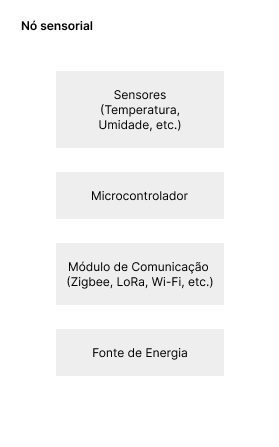
\includegraphics[width=0.5\textwidth]{PFC2/images/no_sensorial.png}
    \label{fig:diagrama}
    \caption*{Fonte: Autor}
\end{figure}

\section{Sensores} 
Um sensor é um dispositivo que detecta e responde a estímulos do ambiente físico. Na agricultura, os sensores são fundamentais ao monitorar condições como temperatura, umidade, luz e a concentração de gases \cite{weg_sensores_industriais}. Um exemplo notável é o sensor CJMCU-811, que mede a concentração de CO2 no ar, ajudando os agricultores a manter níveis ideais para um crescimento saudável das plantas \cite{sparkfun_ccs811_guide}.

Os sensores como o CJMCU-811 utilizam a tecnologia MOX (Metal Oxide Semiconductor) para detectar gases. Essa tecnologia baseia-se na medição da variação na condutividade de um material semicondutor, que altera suas propriedades em resposta à presença do gás. Esses dispositivos são altamente sensíveis e permitem a coleta de dados em tempo real, tornando-se componentes essenciais em sistemas de monitoramento agrícola. A precisão dos sensores pode ser ajustada conforme necessário, com calibrações periódicas que garantem a confiabilidade dos dados \cite{sparkfun_ccs811_guide}.


\begin{figure}[H]
    \centering
     \caption{Módulo sensor CJMCU-811}
    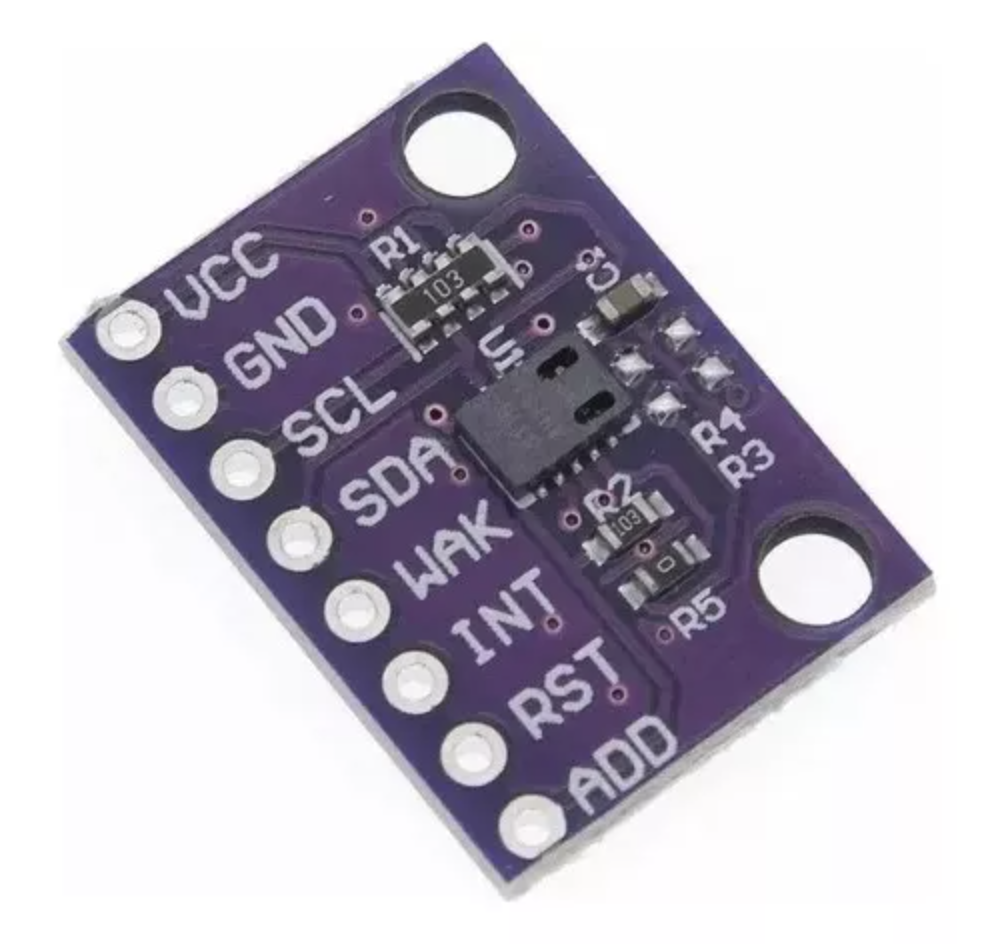
\includegraphics[width=0.3\textwidth]{PFC2/images/sensor.png}
    \label{fig:cjmcu811}

    \caption*{Fonte: Google Imagens}

\end{figure}

A eficiência de um sistema de monitoramento agrícola depende não apenas da qualidade dos sensores, mas também de sua configuração. Para o monitoramento do CO2, a colocação estratégica dos sensores é crucial para garantir a captura de dados representativos. Eles devem operar em diversas condições ambientais, incluindo variações de temperatura e umidade, que são comuns na agricultura \cite{inamasu_agricultura_2011}. Sensores como o CJMCU-811 são projetados para lidar com essas condições, assegurando uma operação estável e precisa \cite{sparkfun_ccs811_guide}.

Outro aspecto relevante é a capacidade de transmissão eficiente dos dados coletados para uma central de controle, exigindo uma integração eficaz com microcontroladores que gerenciam as leituras e enviam os dados pela rede. A compatibilidade entre sensores e microcontroladores, como o ESP8266, é fundamental para garantir que as informações sejam processadas e transmitidas sem perda de qualidade \cite{sparkfun_ccs811_guide}.

Portanto, a escolha de um sensor adequado deve considerar fatores como precisão, condições ambientais, custo e facilidade de manutenção. Um sistema de monitoramento eficiente é construído a partir da seleção correta de sensores e sua integração com a rede de comunicação e o sistema de controle central.


\section{Microcontroladores}

Um microcontrolador é um pequeno computador em um único circuito integrado que contém um processador, memória e periféricos de entrada/saída. Em sistemas de monitoramento agrícola, microcontroladores como o ESP8266 são cruciais para processar os dados coletados pelos sensores e se comunicar com outros dispositivos na rede. O ESP8266 é amplamente utilizado devido à sua capacidade de comunicação via Wi-Fi e baixo consumo de energia, tornando-o ideal para ambientes abertos e remotos \cite{randomnerdtutorials_esp_mesh}.


\begin{figure}[H]
    \centering
     \caption{Microcontrolador ESP8266}
    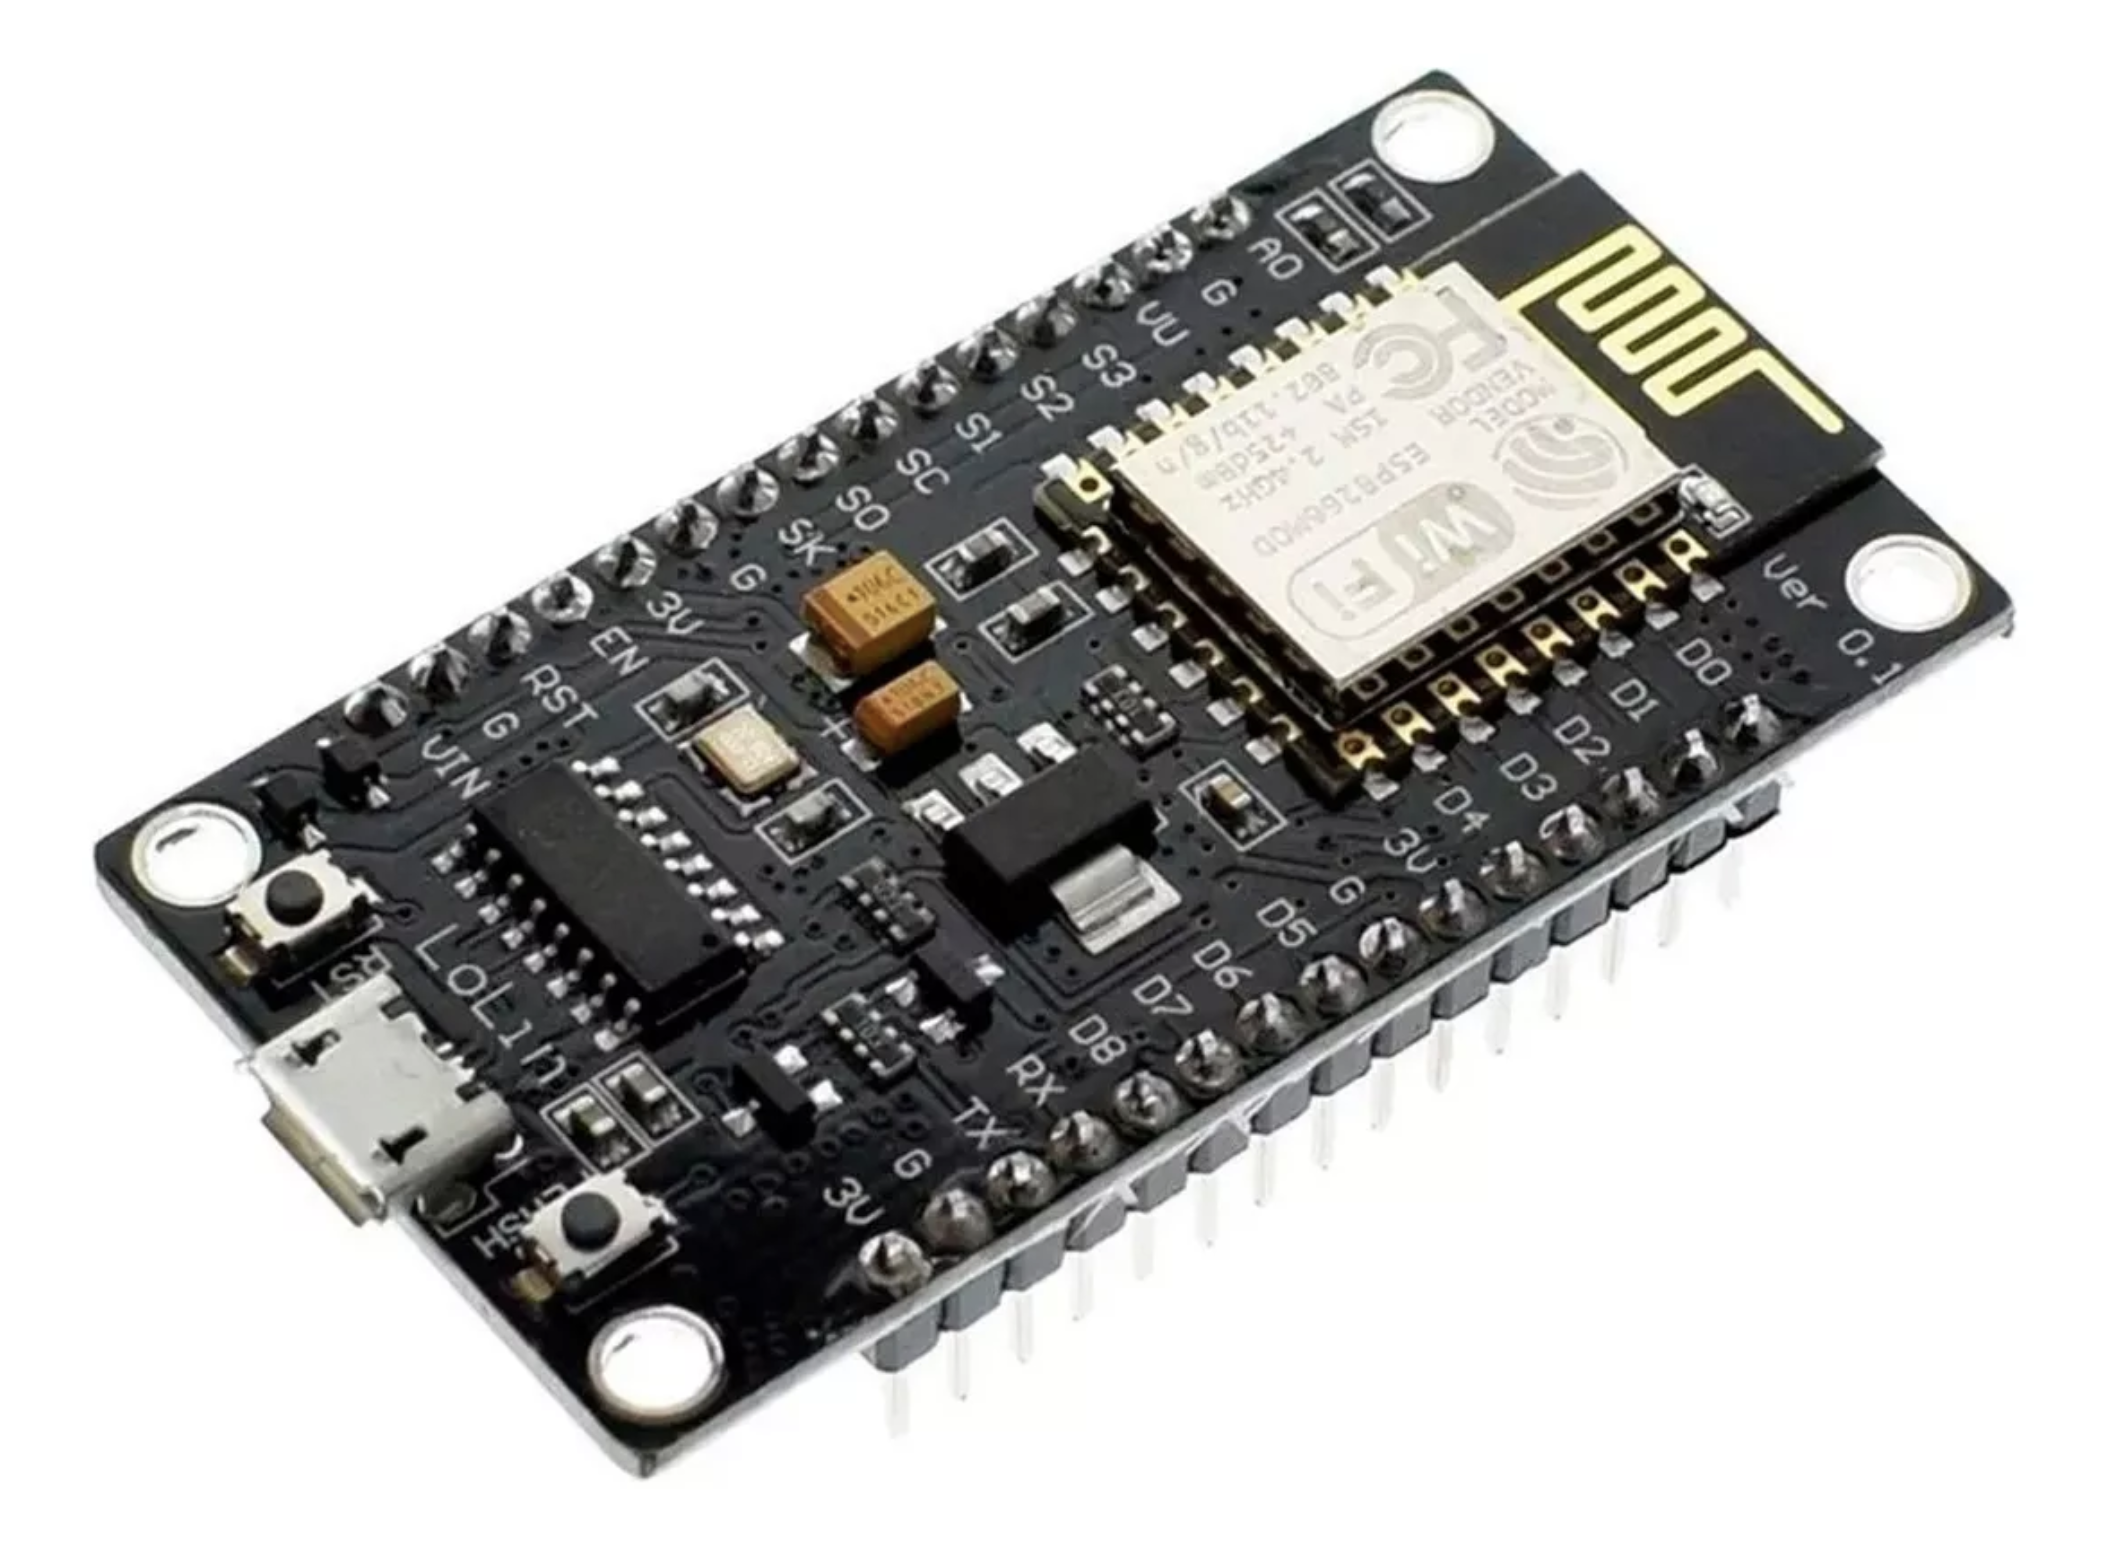
\includegraphics[width=0.5\textwidth]{PFC2/images/microcontrolador.png}
    \label{fig:microcontrolador}
     \caption*{Fonte: Google Images}
\end{figure}

A eficiência energética do ESP8266, que inclui modos de operação de baixo consumo quando inativo, contribui para a prolongação da vida útil das baterias em sistemas de monitoramento distribuídos. Sua conectividade sem fio integrada facilita a comunicação entre nós sensoriais e a central de controle, eliminando a necessidade de infraestrutura complexa e custosa \cite{espressif_esp8266}.

Os microcontroladores são programados para realizar leituras periódicas dos sensores, processar esses dados e transmiti-los a dispositivos ou servidores centrais. A comunicação sem fio via Wi-Fi do ESP8266 permite uma transmissão eficiente em uma rede mesh, garantindo cobertura total em estufas ou campos \cite{espressif_esp8266}. O processamento rápido é essencial para que o sistema responda prontamente a mudanças nas condições ambientais.

Uma vantagem significativa do ESP8266 é a facilidade de integração com diversos tipos de sensores. Ele pode ser configurado para trabalhar diretamente com o sensor CJMCU-811, recebendo dados sobre a concentração de CO2 e transmitindo-os pela rede \cite{randomnerdtutorials_esp_mesh}. Essa flexibilidade torna o ESP8266 uma solução versátil para uma variedade de aplicações agrícolas.

Adicionalmente, o ESP8266 suporta protocolos de comunicação que minimizam o consumo de energia e a latência na transmissão de dados, aspectos essenciais em ambientes com conectividade limitada. Em conjunto com a rede mesh, o microcontrolador assegura um fluxo contínuo de dados entre os nós, mesmo em caso de falhas na rede, aumentando a resiliência do sistema de monitoramento \cite{makerhero}.

O ESP8266 oferece uma solução eficiente para a integração de dispositivos à rede, sendo especialmente útil em projetos de monitoramento ambiental em tempo real. Suas principais características incluem \cite{espressif_esp8266}:

\begin{itemize}
    \item \textbf{Processador:} Tensilica L106 de 32 bits, otimizado para baixo consumo de energia.
    \item \textbf{Memória:} 64 KB de RAM para instruções e 96 KB de RAM para dados.
    \item \textbf{Wi-Fi:} Compatível com os padrões IEEE 802.11 b/g/n, essencial para a comunicação sem fio.
    \item \textbf{Velocidade de Clock:} Até 160 MHz, permitindo processamento rápido para tarefas de coleta e transmissão de dados.
    \item \textbf{Pinos GPIO:} 17 pinos configuráveis, que podem ser utilizados para controlar sensores, relés e LEDs.
    \item \textbf{Interfaces de Comunicação:} Suporte para GPIO, SPI, I2C, UART, I2S, PWM, SDIO e infravermelho (IR), facilitando a comunicação com diversos dispositivos e módulos.
\end{itemize}

\subsection{Pinos de Controle e GPIO}

O ESP8266 possui pinos de controle dedicados e pinos GPIO (entrada e saída digital), que são utilizados para controlar periféricos e sensores:

\begin{itemize}
    \item \textbf{EN (Enable)}: Ativa o microcontrolador quando ligado a 3.3V.
    \item \textbf{RST (Reset):} Reinicia o dispositivo ao ser temporariamente conectado ao GND.
    \item \textbf{CH\_PD (Chip Power Down):} Permite o funcionamento do chip, devendo ser conectado a 3.3V.
\end{itemize}

Os pinos GPIO podem ser configurados como entradas ou saídas digitais, com funcionalidades extras como PWM e comunicação via I2C ou SPI. Por exemplo, o GPIO16 pode ser utilizado para controlar a funcionalidade de "Wake", que acorda o dispositivo.

\subsection{Interfaces de Comunicação}

O ESP8266 oferece várias interfaces de comunicação que permitem a conexão com sensores e outros dispositivos:

\begin{itemize} 
    \item \textbf{UART:} Usado para transmissão e recepção de dados seriais, com pinos TXD0 e RXD0. 
    \item \textbf{SPI:} Interface para comunicação de alta velocidade com dispositivos periféricos, como o CJMCU-811, utilizando os pinos SCLK, MOSI, MISO e CS.
    \item \textbf{I2C:} Interface para conectar sensores via SCL (GPIO5) e SDA (GPIO4), ideal para comunicação com o CJMCU-811. 
    \item \textbf{PWM:} Pinos GPIO12, GPIO13 e GPIO14 suportam PWM, útil para controlar dispositivos externos como motores e LEDs. 
    \item \textbf{ADC:} O pino ADC0 permite a leitura de sinais analógicos de até 1V, possibilitando a integração de outros tipos de sensores. 
\end{itemize}

Essas características tornam o ESP8266 ideal para projetos de monitoramento em tempo real, permitindo a coleta e transmissão eficientes de dados ambientais.

\section{Fontes de Energia}

As fontes de energia são componentes essenciais em um nó sensorial, garantindo que o sistema funcione de maneira autônoma e eficiente. Dependendo da aplicação e da localização do nó, diferentes fontes de energia podem ser utilizadas. As opções mais comuns incluem \cite{espressif_esp8266}:

\begin{enumerate} 
    \item \textbf{Baterias:} Usadas frequentemente em aplicações móveis ou em locais remotos, as baterias oferecem uma solução prática, mas podem exigir substituição ou recarga periódica. 
    \item \textbf{Painéis Solares:} Uma alternativa sustentável e eficiente, especialmente para sistemas de monitoramento ao ar livre. Os painéis solares convertem a luz solar em energia elétrica, permitindo que o nó funcione continuamente sem a necessidade de recarga constante. 
    \item \textbf{Fontes de Energia Híbridas:} Em algumas aplicações, uma combinação de baterias e energia solar pode ser utilizada para garantir que o sistema continue a operar mesmo em dias nublados ou em locais com baixa exposição solar. 
\end{enumerate}

A gestão eficiente da energia é crucial para prolongar a vida útil do nó, especialmente em aplicações remotas onde o acesso a fontes de energia é limitado. Sistemas de monitoramento que implementam técnicas de gerenciamento de energia, como modos de baixo consumo e ciclos de sono, podem maximizar a eficiência e a durabilidade dos componentes.

\section{Módulos de Comunicação}

Os módulos de comunicação são responsáveis pela conectividade entre o nó sensorial e a rede Mesh. Eles permitem que os dados coletados pelos sensores sejam transmitidos para outros nós ou para um servidor central. As opções mais comuns de módulos de comunicação incluem \cite{espressif_esp8266}:

\begin{enumerate} 
    \item \textbf{Wi-Fi:} Proporciona uma conexão de alta velocidade e é ideal para ambientes onde a infraestrutura de rede já existe. O ESP8266, por exemplo, possui comunicação Wi-Fi integrada, facilitando a transmissão de dados. 
    \item \textbf{Zigbee:} Uma tecnologia de comunicação sem fio projetada para aplicações de baixo consumo de energia e alcance limitado, ideal para redes de sensores em ambientes agrícolas. 
    \item \textbf{LoRa:} Oferece longa distância de transmissão com baixo consumo de energia, sendo particularmente útil em áreas rurais extensas onde a cobertura de rede é limitada. 
    \item \textbf{Bluetooth:} Pode ser usado para comunicação de curto alcance, sendo útil em aplicações onde dispositivos móveis estão envolvidos na coleta ou visualização de dados. 
\end{enumerate}

A escolha do módulo de comunicação adequado depende das necessidades específicas do sistema, como alcance, largura de banda e consumo de energia.


\section{Armazenamento Local}

Em algumas implementações \cite{vidadesilicio_nodemcu_sd_module}, o nó sensorial pode incluir um meio de armazenamento local, como um cartão SD ou memória flash, para armazenar temporariamente os dados coletados antes da transmissão. Essa funcionalidade é particularmente útil em cenários onde a conectividade com a rede pode ser intermitente ou quando é necessário realizar análises locais antes de enviar os dados.

O armazenamento local permite que os dados sejam mantidos até que uma conexão adequada esteja disponível, garantindo que nenhuma informação crítica seja perdida. Além disso, pode ser usado para armazenar configurações do sistema e registros de operação, facilitando a manutenção e o diagnóstico de falhas.

A inclusão de armazenamento local em um nó sensorial aumenta a resiliência do sistema, permitindo que ele opere de maneira eficaz, mesmo em condições de conectividade limitada ou instável.

\section{Funcionamento do Nó Sensorial}
O funcionamento do nó sensorial envolve uma sequência coordenada de etapas que garantem a coleta eficiente de dados ambientais, seu processamento e a comunicação adequada com outros componentes do sistema. Essas etapas são essenciais para permitir um monitoramento confiável e contínuo. As principais etapas incluem:

\subsection{Coleta de Dados}

O processo começa com a coleta de dados realizada pelos sensores, que capturam variáveis ambientais como temperatura, umidade, concentração de dióxido de carbono, luminosidade, entre outras. Cada sensor é responsável por monitorar um aspecto específico do ambiente, que pode ser crucial para o crescimento e a saúde das plantas. Por exemplo:

\begin{itemize}
    \item Um sensor de temperatura mede a temperatura ambiente a intervalos regulares, permitindo o controle do clima em uma estufa.
    \item Um sensor de umidade do solo verifica se as plantas têm água suficiente, acionando sistemas de irrigação automaticamente quando necessário.
    \item Um sensor de CO2 mede a concentração de dióxido de carbono para garantir que os níveis estejam adequados para a fotossíntese.
\end{itemize}

A frequência de amostragem dos sensores é configurada com base nas necessidades da aplicação, equilibrando a precisão dos dados e o consumo de energia.

\subsection{Processamento dos Dados}

Após a coleta, os dados são enviados ao microcontrolador para processamento. Esse processamento envolve várias operações:
\begin{itemize}
    \item \textbf{Filtragem de ruídos:} Pode haver interferências nos dados coletados, como medições esporádicas que estão fora dos padrões esperados. Técnicas de filtragem, como a média móvel, são aplicadas para remover esses ruídos.
    \item \textbf{Conversão de unidades:} Alguns sensores retornam valores em formatos que precisam ser convertidos. Por exemplo, a leitura de um sensor de umidade pode precisar ser transformada em porcentagem.
    \item \textbf{Tomada de decisão:} O microcontrolador pode decidir se os dados são relevantes o suficiente para serem transmitidos. Por exemplo, ele pode programar para enviar dados apenas quando houver uma mudança significativa nas condições monitoradas. Isso ajuda a economizar energia e recursos de comunicação.
\end{itemize}

Além disso, os microcontroladores podem agregar dados para criar resumos úteis, como médias diárias ou alertas sobre mudanças rápidas que possam afetar o cultivo.

\subsection{Comunicação com a Rede Mesh}

Com os dados processados, o nó sensorial passa para a etapa de comunicação com a rede Mesh. A rede Mesh é uma infraestrutura distribuída em que cada nó atua como um retransmissor, permitindo a comunicação eficiente mesmo em áreas onde uma conexão direta com um gateway seria difícil.

A escolha do protocolo de comunicação, como Zigbee, Wi-Fi ou LoRa, depende das características do ambiente agrícola:
\begin{itemize}
    \item Em áreas onde se requer cobertura de longo alcance, o LoRa é preferido devido ao seu alcance maior e baixo consumo de energia.
    \item Para áreas menores ou que já possuam infraestrutura de Wi-Fi, o ESP8266 é uma escolha prática, oferecendo comunicação sem fio com baixo custo.
\end{itemize}

Uma característica importante da rede Mesh é sua resiliência: se um nó falhar, os outros encontram rotas alternativas, garantindo a continuidade da comunicação. Essa propriedade é fundamental em ambientes adversos como campos agrícolas.

\subsection{Transmissão de Dados para o Gateway ou Servidor Central}

Depois de se comunicar com a rede Mesh, o próximo passo é a transmissão dos dados para um nó pai, que pode ser um gateway ou um servidor central. Este nó é responsável por consolidar as informações vindas de diferentes nós sensoriais e armazená-las para análises posteriores.

O servidor central pode realizar análises em tempo real ou armazenar os dados para posterior análise histórica, ajudando os agricultores a entenderem padrões de crescimento e identificar problemas. A centralização dos dados também possibilita a integração com outras plataformas, como sistemas de automação que ajustam automaticamente os parâmetros ambientais.

\subsection{Gerenciamento de Energia}

O gerenciamento de energia é uma parte crucial do funcionamento do nó sensorial, especialmente em ambientes onde a energia elétrica não está disponível. Para garantir uma operação autônoma e prolongada, os nós utilizam várias estratégias:
\begin{itemize}
    \item \textbf{Modos de baixa potência:} O microcontrolador entra em um estado de baixo consumo quando não está realizando leituras ou transmitindo dados. Sensores e microcontroladores geralmente trabalham em ciclos de sono e acordam apenas em intervalos pré-programados.
    \item \textbf{Uso de fontes renováveis:} Sistemas movidos a painéis solares são comuns em ambientes agrícolas. Durante o dia, os painéis solares carregam baterias, garantindo que os sensores funcionem de forma contínua, mesmo à noite.
    \item \textbf{Balanceamento de carga entre nós:} Na rede Mesh, os nós podem compartilhar a tarefa de retransmissão de dados, evitando que um nó específico consuma toda a sua energia rapidamente.
\end{itemize}

Um exemplo prático de gerenciamento de energia envolve a combinação de sensores que coletam dados apenas em momentos específicos do dia. Por exemplo, medições da concentração de CO2 podem ser feitas em horários de maior fotossíntese, enquanto a temperatura e umidade do solo são monitoradas em intervalos regulares.

\subsection{Monitoramento e Ajustes Remotos}

Os nós sensoriais também permitem monitoramento e ajustes remotos. Utilizando plataformas de gerenciamento na nuvem, agricultores podem acessar dados em tempo real através de dispositivos móveis ou computadores, ajustando parâmetros como frequência de coleta ou calibrando sensores sem precisar estar fisicamente presentes. Isso é particularmente útil para responder a eventos críticos, como mudanças bruscas de temperatura, que exigem uma ação rápida.

\subsection{Automação Baseada em Dados}

Além do monitoramento, o sistema de nós sensoriais pode ser integrado a atuadores, como sistemas de irrigação ou ventilação. Quando os sensores detectam condições específicas (por exemplo, níveis de umidade abaixo do limite), o microcontrolador pode ativar automaticamente os atuadores, realizando ajustes no ambiente sem intervenção humana.

\section{Considerações finais}

Para finalizar o capítulo sobre o nó sensorial, podemos destacar a relevância e os desafios envolvidos no desenvolvimento e implementação desse componente em sistemas de monitoramento ambiental, especialmente na agricultura.

O nó sensorial é uma peça fundamental na coleta de dados ambientais de forma precisa e contínua, fornecendo informações essenciais para a análise das emissões de CO2 em tempo real. A integração de sensores, microcontroladores e módulos de comunicação permite a obtenção de dados em diferentes locais do campo, de maneira automatizada e eficiente, viabilizando uma resposta mais rápida e informada para a mitigação de impactos climáticos.

Além disso, o uso de redes Mesh e protocolos de comunicação como Zigbee e LoRa torna os nós sensoriais robustos e resilientes, garantindo que as informações coletadas cheguem de forma confiável aos centros de processamento. No entanto, é importante reconhecer que o gerenciamento de energia e a adaptação às condições do ambiente são desafios contínuos que exigem soluções inteligentes para garantir a durabilidade e a eficiência do sistema.

Assim, o nó sensorial se apresenta como um elemento essencial para a agricultura moderna e sustentável, contribuindo significativamente para a redução das emissões de gases de efeito estufa e para o aumento da produtividade. Com o avanço das tecnologias de sensores e microcontroladores, espera-se que esses dispositivos possam ser cada vez mais eficientes, acessíveis e aplicáveis a uma gama maior de cenários agrícolas.

\postextual

\bibliography{references}

\input{tex/glossario}
\glsaddall
\printglossaries

\end{document}